\documentclass[11pt]{article}\usepackage[]{graphicx}\usepackage[]{color}
% maxwidth is the original width if it is less than linewidth
% otherwise use linewidth (to make sure the graphics do not exceed the margin)
\makeatletter
\def\maxwidth{ %
  \ifdim\Gin@nat@width>\linewidth
    \linewidth
  \else
    \Gin@nat@width
  \fi
}
\makeatother

\definecolor{fgcolor}{rgb}{0.345, 0.345, 0.345}
\newcommand{\hlnum}[1]{\textcolor[rgb]{0.686,0.059,0.569}{#1}}%
\newcommand{\hlstr}[1]{\textcolor[rgb]{0.192,0.494,0.8}{#1}}%
\newcommand{\hlcom}[1]{\textcolor[rgb]{0.678,0.584,0.686}{\textit{#1}}}%
\newcommand{\hlopt}[1]{\textcolor[rgb]{0,0,0}{#1}}%
\newcommand{\hlstd}[1]{\textcolor[rgb]{0.345,0.345,0.345}{#1}}%
\newcommand{\hlkwa}[1]{\textcolor[rgb]{0.161,0.373,0.58}{\textbf{#1}}}%
\newcommand{\hlkwb}[1]{\textcolor[rgb]{0.69,0.353,0.396}{#1}}%
\newcommand{\hlkwc}[1]{\textcolor[rgb]{0.333,0.667,0.333}{#1}}%
\newcommand{\hlkwd}[1]{\textcolor[rgb]{0.737,0.353,0.396}{\textbf{#1}}}%
\let\hlipl\hlkwb

\usepackage{framed}
\makeatletter
\newenvironment{kframe}{%
 \def\at@end@of@kframe{}%
 \ifinner\ifhmode%
  \def\at@end@of@kframe{\end{minipage}}%
  \begin{minipage}{\columnwidth}%
 \fi\fi%
 \def\FrameCommand##1{\hskip\@totalleftmargin \hskip-\fboxsep
 \colorbox{shadecolor}{##1}\hskip-\fboxsep
     % There is no \\@totalrightmargin, so:
     \hskip-\linewidth \hskip-\@totalleftmargin \hskip\columnwidth}%
 \MakeFramed {\advance\hsize-\width
   \@totalleftmargin\z@ \linewidth\hsize
   \@setminipage}}%
 {\par\unskip\endMakeFramed%
 \at@end@of@kframe}
\makeatother

\definecolor{shadecolor}{rgb}{.97, .97, .97}
\definecolor{messagecolor}{rgb}{0, 0, 0}
\definecolor{warningcolor}{rgb}{1, 0, 1}
\definecolor{errorcolor}{rgb}{1, 0, 0}
\newenvironment{knitrout}{}{} % an empty environment to be redefined in TeX

\usepackage{alltt}

\usepackage{rotating}
\usepackage{graphics}
\usepackage{latexsym}
\usepackage{color}
\usepackage{listings}
\usepackage{wrapfig}
\usepackage{float}
\usepackage[belowskip=-15pt,aboveskip=0pt]{caption}

\setlength\topmargin{-.56in}
\setlength\evensidemargin{0in}
\setlength\oddsidemargin{0in}
\setlength\textwidth{6.49in}
\setlength\textheight{8.6in}
\setlength{\intextsep}{10pt plus 1pt minus 4pt}

\definecolor{codegreen}{rgb}{0,0.6,0}
\definecolor{codegray}{rgb}{0.5,0.5,0.5}
\definecolor{codepurple}{rgb}{0.58,0,0.82}
\definecolor{backcolour}{rgb}{0.95,0.95,0.92}
\lstdefinestyle{mystyle}{
	backgroundcolor=\color{backcolour},   
	commentstyle=\color{codegreen},
	keywordstyle=\color{magenta},
	numberstyle=\tiny\color{codegray},
	stringstyle=\color{codepurple},
	basicstyle=\footnotesize,
	breakatwhitespace=false,         
	breaklines=true,                 
	captionpos=b,                    
	keepspaces=true,                 
	numbers=left,                    
	numbersep=5pt,                  
	showspaces=false,                
	showstringspaces=false,
	showtabs=false,                  
	tabsize=2
}
\lstset{style=mystyle}

\pagestyle{headings}

\title{Predictive Model for Average Avocado Prices\vspace{-5ex}} 
\date{December 16, 2020\vspace{-5ex}}
\IfFileExists{upquote.sty}{\usepackage{upquote}}{}
\begin{document} 
\maketitle
\hfill \break
















\noindent\textbf{\underline{Executive Summary}}:      
\hfill \break

\noindent\textbf{\underline{Introduction}}: Avocado is a fruit that is originated from southern America. This fruit is extremaly health and have a lot of benefits and nutritions. Individuals can use avocados with any other ingridients to complete a meal such as toast and salad. In addition, avocados can also be used to make healthy oil or desserts like avocado ice cream or smoothie. Knowing the fact that avocados are health for a human body, avocados have been the rise of American's new favorites fruits since the last decade. The amount of avocados have been sold in America are higher and higher everyday. With this being said, knowing the variables that cause the price of avocados to go up and down would benefits all consumers and restaurants owner. For example, a restaurants that have avocado toast or guacamole on their menu would have a better understanding of where to get cheaper avocados to maximize their profit. Knowing the cost of avocado can also help restaurants owner create budget for their restaurant and cost of a dish on their menu. In addition, individuals who like avocado would also know where and when to get type of avocado they desire. There are many questions asked in favor of these issues including 1) What factor impact the average price of avocados? 2) Are characteristics of an avocado important in pricing decision? 3) How good is the model? 4) How can we improve the model? and 5) How can we implement the model for the consumer to gain easy access? This analysis will attempt to answer all these questions by starting with a variable data analysis, developing the model using a multiple linear regression, assessing the quality of the model, and providing significant results of the model. The purpose of this model is to predict the average avocado prices using various variables provided in the dataset.         
\hfill \break

\noindent\textbf{\underline{Methods}}: A dataset was retrieved from Kaggle, a website that have input and output from scientists and college students. This dataset has a large sample size of 30,021 observations from 2015 to 2020. The data was originally collected from the Hass Avocado Broad (HAB) website. There are no missing values for all the variables in the dataset. This dataset has historical data of avocado prices and characteristics. The dataset contains two time series columns including date of observation and year of observation, one characteristic variable including type of the avocado, and one geographical variable. In addition, there are eight quantitative predictors including total number of avocados sold, total number of avocados with Price Look-Up (PLU) code 4046 sold, total number of avocados with PLU code 4226 sold, total number of avocados with PLU code 4770 sold, total number of bags sold, total number of small bags sold, total number of large bags sold, and total number of extra large bags sold. There are 54 distinct geographical regions of where the avocados are from with different average prices for different time of the year. The goal of this analysis is to find the relationship between predictors and average avocado prices. To build a model with average avocado price, a multiple linear regression with signficant predictors will be used. Before building a model, we will explore how each variable impact the average of avocado prices. Then, using the "best" model, we will predict the avocado price to validate our model. All analysis will be done in R Studio with version 3.6.2.  
\hfill \break

\noindent\textbf{\underline{Exploratory Data Analysis}}: Before building a model, it is important to explore the distribution of average avocado prices and the relationship of it with each of the predictor.  

\begin{figure}[h!] 
\begin{center}

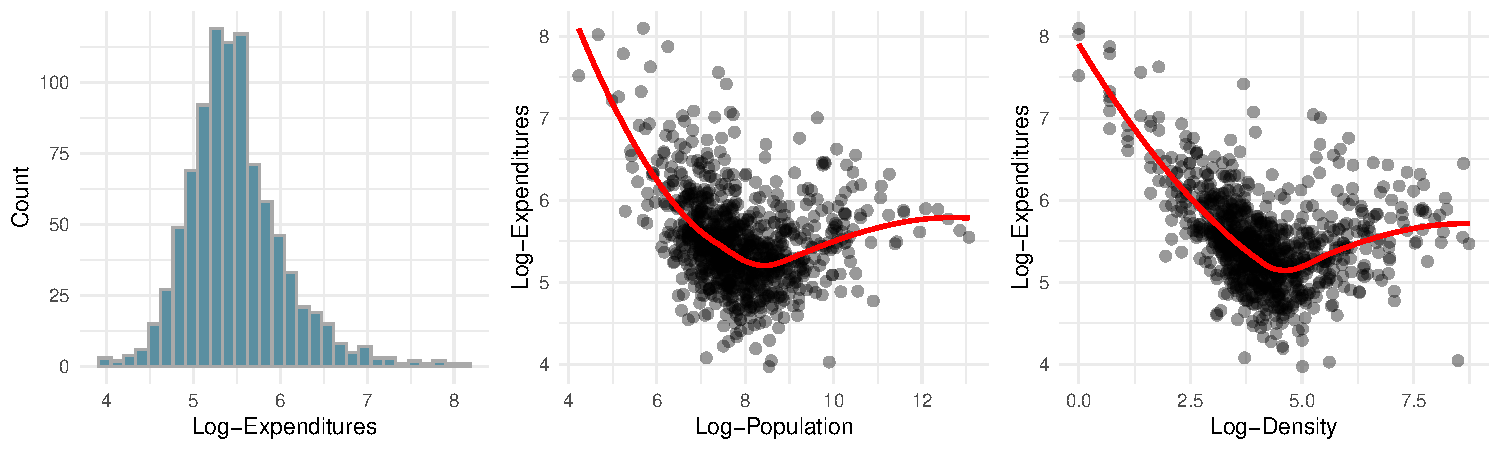
\includegraphics[width=\maxwidth]{figure/unnamed-chunk-1-1} 

\caption{}
\label{explore1}
\end{center} 
\end{figure}


\begin{figure}[h!] 
\begin{center}

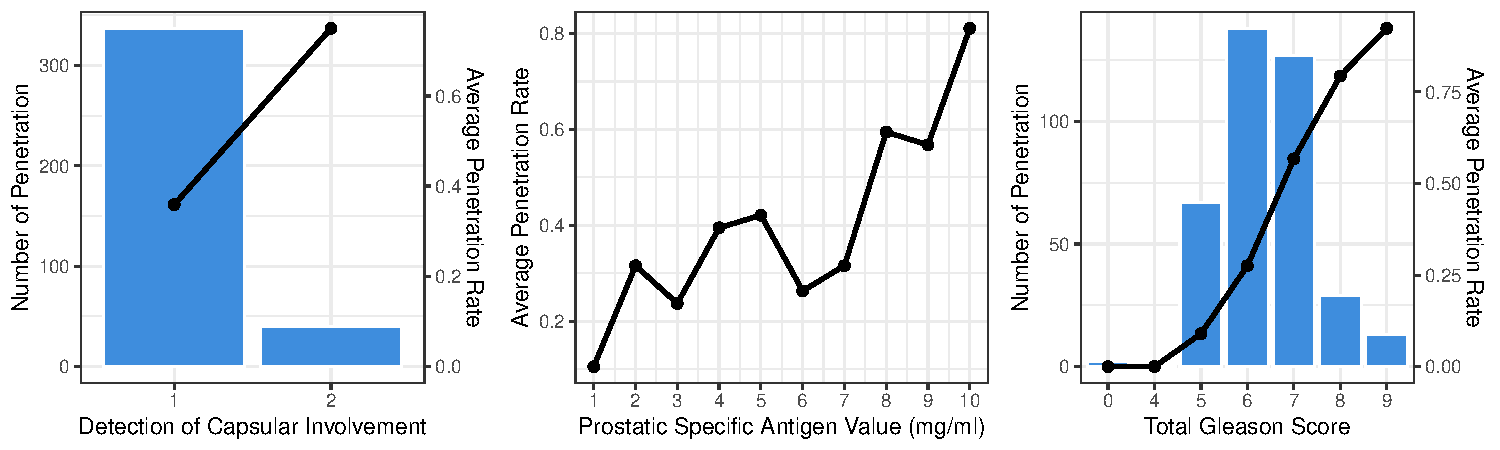
\includegraphics[width=\maxwidth]{figure/unnamed-chunk-2-1} 

\caption{}
\label{explore2}
\end{center} 
\end{figure}


\begin{figure}[h!] 
\begin{center}

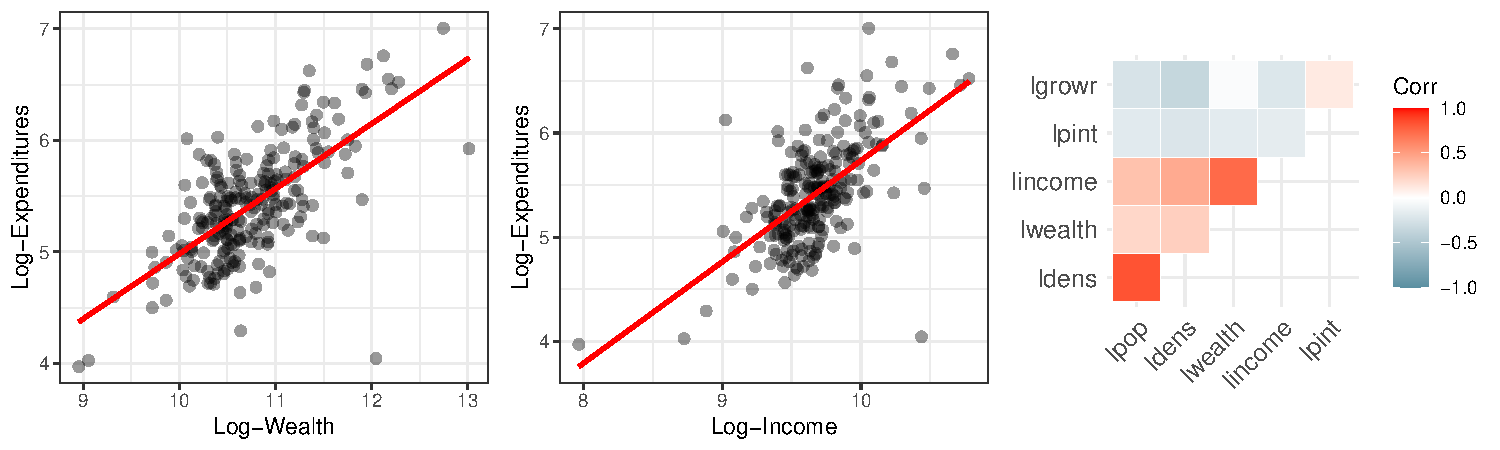
\includegraphics[width=\maxwidth]{figure/unnamed-chunk-3-1} 

\caption{}
\label{explore3}
\end{center} 
\end{figure}





\begin{center}
% latex table generated in R 3.6.2 by xtable 1.8-4 package
% Sun Dec 13 15:35:58 2020
\begin{table}[ht]
\centering
\begin{tabular}{lrrrrrr}
  \hline
Term & Coef & SdError & F-Stat & pValue & 2.5\% CI & 97.5\% CI \\ 
  \hline
(Intercept) & 1.228 & 0.018 & 70.111 & 0.000 & 1.193 & 1.262 \\ 
  log\_total\_volume & -0.029 & 0.001 & -23.237 & 0.000 & -0.031 & -0.026 \\ 
  month2 & -0.037 & 0.008 & -4.712 & 0.000 & -0.052 & -0.021 \\ 
  month3 & 0.031 & 0.008 & 4.066 & 0.000 & 0.016 & 0.045 \\ 
  month4 & 0.094 & 0.008 & 12.402 & 0.000 & 0.079 & 0.109 \\ 
  month5 & 0.080 & 0.008 & 10.502 & 0.000 & 0.065 & 0.095 \\ 
  month6 & 0.134 & 0.008 & 16.547 & 0.000 & 0.118 & 0.149 \\ 
  month7 & 0.198 & 0.008 & 25.137 & 0.000 & 0.182 & 0.213 \\ 
  month8 & 0.223 & 0.008 & 27.667 & 0.000 & 0.207 & 0.239 \\ 
  month9 & 0.242 & 0.008 & 30.527 & 0.000 & 0.227 & 0.258 \\ 
  month10 & 0.192 & 0.008 & 24.207 & 0.000 & 0.176 & 0.207 \\ 
  month11 & 0.113 & 0.008 & 13.961 & 0.000 & 0.097 & 0.129 \\ 
  month12 & 0.026 & 0.008 & 3.202 & 0.001 & 0.010 & 0.043 \\ 
  typeorganic & 0.367 & 0.005 & 67.379 & 0.000 & 0.356 & 0.377 \\ 
  geography\_bins2 & 0.160 & 0.005 & 33.397 & 0.000 & 0.150 & 0.169 \\ 
  geography\_bins3 & 0.309 & 0.005 & 61.764 & 0.000 & 0.299 & 0.318 \\ 
  geography\_bins4 & 0.563 & 0.008 & 69.124 & 0.000 & 0.547 & 0.579 \\ 
   \hline
\end{tabular}
\caption{Summary regression of final model} 
\label{final_fit}
\end{table}

\end{center}








\begin{figure}[h!] 
\begin{center}

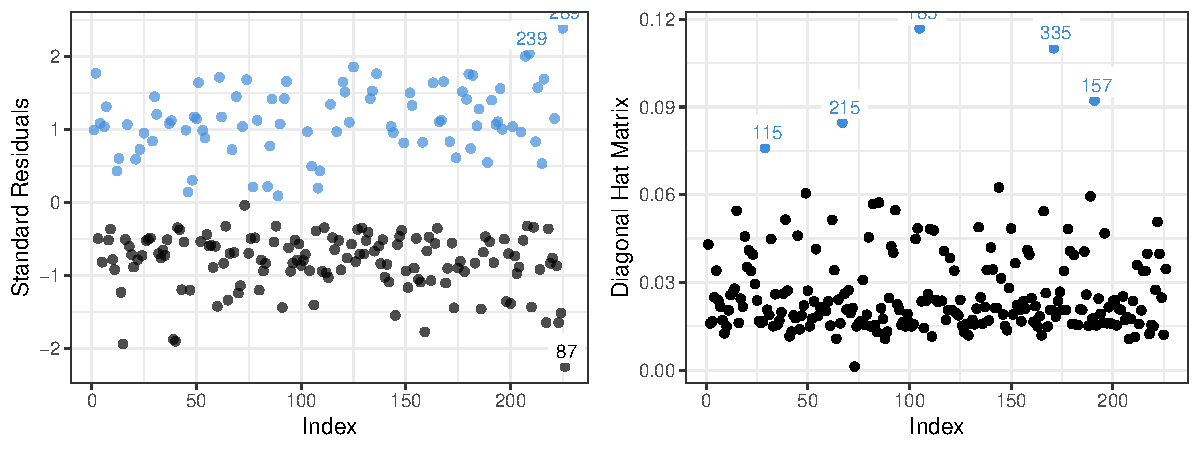
\includegraphics[width=\maxwidth]{figure/unnamed-chunk-5-1} 

\caption{}
\label{explore3}
\end{center} 
\end{figure}


\begin{figure}[h!] 
\begin{center}

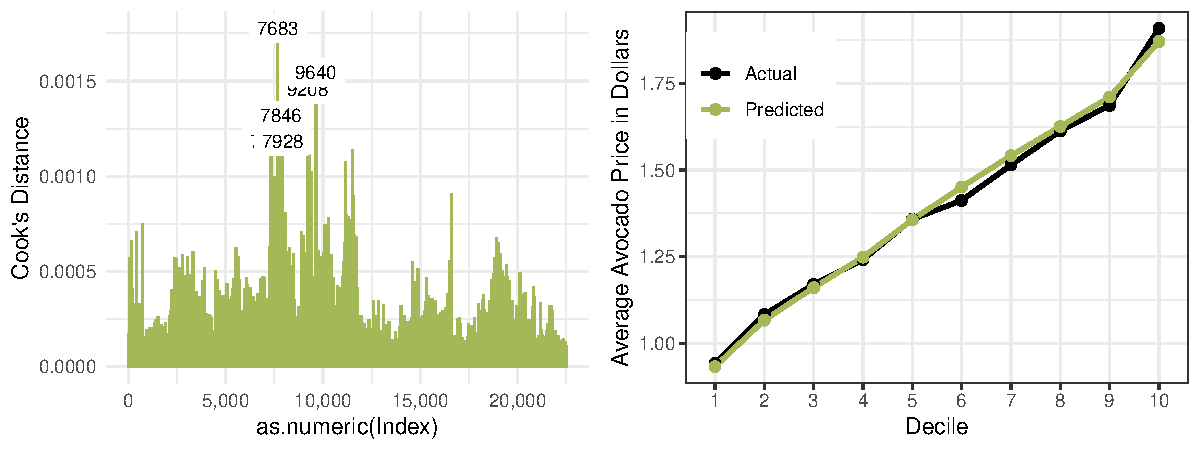
\includegraphics[width=\maxwidth]{figure/unnamed-chunk-6-1} 

\caption{}
\label{explore3}
\end{center} 
\end{figure}


\noindent\textbf{\underline{Model Fitting/Inferences}}: 
\hfill \break

\noindent\textbf{\underline{Conclusion}}: 
\hfill \break


\clearpage
\noindent\textbf{\underline{Introduction}}:
\hfill \break


\clearpage
\newpage
\noindent \Large{{\bf Appendix A: Supplemental Tables}}

\begin{center}

% Table created by stargazer v.5.2.2 by Marek Hlavac, Harvard University. E-mail: hlavac at fas.harvard.edu
% Date and time: Sun, Dec 13, 2020 - 3:36:08 PM
\begin{table}[H] \centering 
  \caption{Summary Statistics for all numerical independent features} 
  \label{} 
\begin{tabular}{@{\extracolsep{5pt}}lccccccc} 
\\[-1.8ex]\hline 
\hline \\[-1.8ex] 
Statistic & \multicolumn{1}{c}{N} & \multicolumn{1}{c}{Mean} & \multicolumn{1}{c}{St. Dev.} & \multicolumn{1}{c}{Min} & \multicolumn{1}{c}{Pctl(25)} & \multicolumn{1}{c}{Pctl(75)} & \multicolumn{1}{c}{Max} \\ 
\hline \\[-1.8ex] 
total\_volume & 30,021 & 939,255 & 3,813,519 & 85 & 14,299 & 489,803 & 63,716,144 \\ 
4046 & 30,021 & 299,107 & 1,289,108 & 0 & 783 & 115,156 & 22,743,616 \\ 
4225 & 30,021 & 284,901 & 1,169,078 & 0 & 2,814 & 140,947 & 20,470,573 \\ 
4770 & 30,021 & 21,629 & 100,919 & 0 & 0 & 5,424 & 2,546,439 \\ 
total\_bags & 30,021 & 333,534 & 1,415,618 & 0 & 8,374 & 159,174 & 31,689,189 \\ 
small\_bags & 30,021 & 232,126 & 950,503 & 0 & 5,956 & 112,938 & 20,550,407 \\ 
large\_bags & 30,021 & 95,185 & 467,210 & 0 & 352 & 36,068 & 13,327,601 \\ 
xlarge\_bags & 30,021 & 6,223 & 38,137 & 0 & 0 & 560 & 1,022,564 \\ 
\hline \\[-1.8ex] 
\end{tabular} 
\end{table} 

\end{center}

\begin{center}
% latex table generated in R 3.6.2 by xtable 1.8-4 package
% Sun Dec 13 15:36:08 2020
\begin{table}[ht]
\centering
\begin{tabular}{rp{1.5in}p{.8in}llll}
  \hline
 & Model & Number of Features & MSE & Adj.R.squared & F.statistics & AIC \\ 
  \hline
1 & Initial Model & 16.000 & 0.062 & 0.572 & 1879.873 & 1421.841 \\ 
  2 & Stepwise Model & 16.000 & 0.062 & 0.572 & 1879.873 & 1421.841 \\ 
  3 & Model with Interaction Terms & 78.000 & 0.060 & 0.588 & 413.437 & 598.507 \\ 
  4 & Stepwise Model with Interaction Terms & 77.000 & 0.060 & 0.588 & 418.808 & 597.053 \\ 
   \hline
\end{tabular}
\caption{Regression validation metrics including MSE, R-squared adjusted, and AIC} 
\label{reg_vali_metric}
\end{table}

\end{center} 


\begin{center}
% latex table generated in R 3.6.2 by xtable 1.8-4 package
% Sun Dec 13 15:36:08 2020
\begin{table}[ht]
\centering
\begin{tabular}{rrrr}
  \hline
 & GVIF & Df & GVIF\verb|^|(1/(2*Df)) \\ 
  \hline
log\_total\_volume & 2.713 & 1.000 & 1.647 \\ 
  month & 1.007 & 11.000 & 1.000 \\ 
  type & 2.673 & 1.000 & 1.635 \\ 
  geography\_bins & 1.031 & 3.000 & 1.005 \\ 
   \hline
\end{tabular}
\caption{} 
\label{vif_table}
\end{table}

\end{center} 

\clearpage
\newpage
\noindent \Large{{\bf Appendix B: R Code}}
\lstinputlisting[language=R, caption = Appendix of Code]{R/dar3-codes.R}


\end{document}






